%----------------------------------------------------------------------------------------
%	APPAENDIX : FOCUS SURFACES
%----------------------------------------------------------------------------------------
%\section{Reconstruction of the focus surfaces}
%\label{sec:focus_surfaces}

Owing to the NIKA2 $6.5~\rm{arcmin}$ FOV, the focus is expected to
slightly changes across the FOV, defining curved focal surfaces at the
location of the three arrays. Therefore, beam patterns are expected to
show some scatter across the FOV accordingly to the focal
surfaces. Although all the detectors cannot be individually focalised,
an optimal axial focus of the telescope can be found to maximize the
number of detectors at the best focus and hence, maximize the
resolution of the NIKA2 maps.
This optimal z-focus setting is obtained by measuring the focus at the center of the arrays as described
Sect.~\ref{se:axial_focus} and apply a focus shift, which is primary
predicted using ZEMAX simulations, and ultimately verified by measuring
the focus surfaces as decribed here.

\begin{figure*}[!thbp]
\begin{center}
  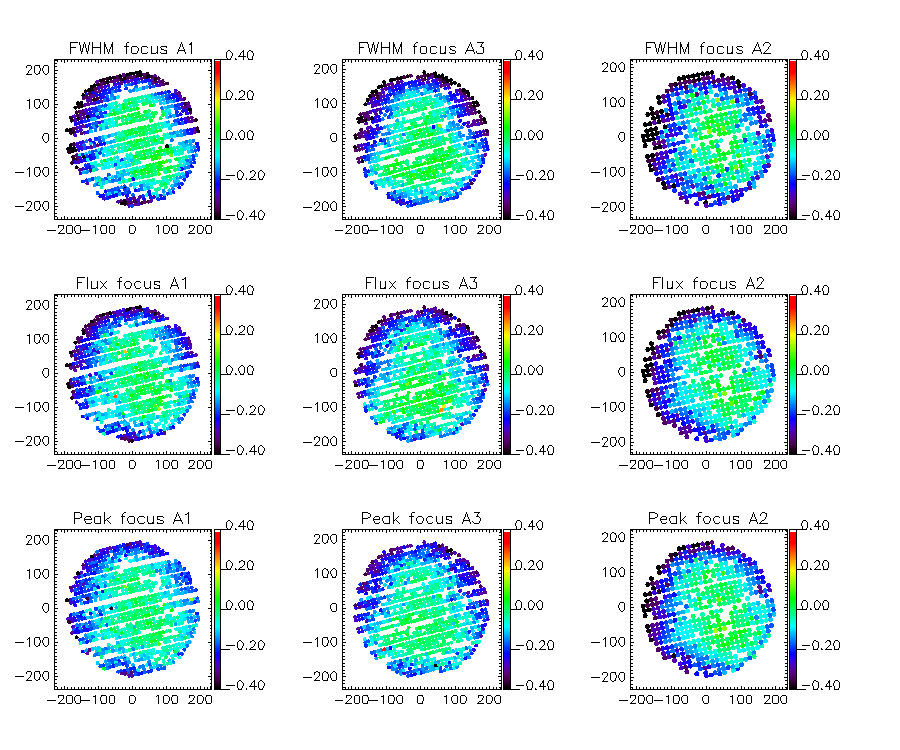
\includegraphics[trim={0, 9.5cm, 0, 9.5cm}, clip=true, width=\linewidth]{Figures/fov_focus_mv_5.png}
\caption[Focus surfaces]{Focus surface of A1, A3 and A2 arrays from left to
  right. From top to bottom, the focus estimates rely on
  FWHM-minimization, amplitude-maximization of a 2D
  Gaussian of fixed FWHMs and amplitude-maximization of an elliptical
  Gaussian. On each plot, the x and y axis are the Nasmyth offsets
  w.r.t. the center of the array in arcsec, while the color-code represents
  the relative focus estimate w.r.t. the central focus, given in mm.}
\label{fig:focus-surfaces}
\end{center}
\end{figure*}

\subsection{Method}

We estimate NIKA2 focal surfaces by means of a sequence of five
defocused \bms\ of bright
point-like sources, typically planets or bright quasars, for various settings of
the telescope axial focus around the optimal focus $z_{\rm{opt}}$.
The z-focus is changed in step of $0.6~\rm{mm}$ to probe a large
focus range for measuring even the extreme variation of the focus surfaces,
namely $z \in \{-1.2, -0.6, 0, 0.6, 1.2 \} + z_{\rm{opt}}$.  Each
\bm\ is analysed using the data reduction pipeline, as described in
Sect.~\ref{se:pipeline_overview}, and $4''$-resolution individual maps per KID
are projected. 
Therefore, a series of
five cleaned maps at various focus is available for each detector, from which
the best focus is estimated as described in Sect.~\ref{se:axial_focus}. The
ensemble of the relative focus estimate per KIDs with respect to the best focus
at the center of the array constitutes the focus surface. An accurate estimate
of the center focus is obtained as the weighted average focus estimate of the
KIDs lying in a $30''$ radius around the geometrical center of the array. This
average does not induce any sizeable bias thanks to the flatness of the focus
surface in the innermost regions. For robustness test, we consider three focus
estimates: the two first ones are the same as discussed in
Sect.~\ref{se:axial_focus} -- namely i) $\hat z_{\rm{fwhm}}$ the focus that
minimizes the geometrical FWHM and ii) $\hat z_{\rm{peak}}$ the focus that
maximizes the amplitude of the best-fitting elliptical Gaussian -- whereas the
third one is $\hat z_{\rm{flux}}$ the focus that maximizes the amplitude of the
best-fitting Gaussian of fixed FWHM (at $12.5''$ at $260~\rm{GHz}$ and
$18.5''$ at $150~\rm{GHz}$). The comparison between the two amplitude-based
estimators ($\hat z_{\rm{peak}}$ and $\hat z_{\rm{flux}}$), will test the
stability of the focus results against the exact choice of the beam fitting
function. Since the ellipticity-based estimator $\hat z_{\rm{ellip}}$ is less
sensitive to focus changes and yields larger uncertainties than the others, we
do not use it for the focus surface reconstruction.


\subsection{Data set}

%After the change of A1 lens and the improvement of internal optics
%alignment (hence in the final NIKA2 optical configuration) that is
%during the N2R8 two-day run, N2R9 and N2R10,
In the final NIK2 optical configuration, 
nine defocused \bm\ sequences have been acquired, including incomplete
sequences and sequences hindered by poor atmospheric conditions.
We select sequences that i) comprises at least four scans, ii) have been
observed at zenith opacity at $225\,\rm{GHz}$ (as indicated by
the IRAM \taumeter) below 0.5 and iii) have a maximal central focus
drift between the starting time and the end of the sequence of
$0.5~\rm{mm}$. These criteria preserve five sequences from which focus
surfaces can be reconstructed %. Namely, we consider the sequences
%$20170226s415\mbox{--}419$, $20170419s133\mbox{--}137$, $20170420s113\mbox{--}117$,
%$20170421s160\mbox{--}164$ and $20170424s123\mbox{--}127$, which consist of observations
%of the bright quasar 3C84 and Neptune.
and that correspond to observations of the bright quasar 3C84 and Neptune.

\subsection{Results}
For each detector $k$ and for each \bm\ sequence $s$, we obtain for
the array $a$, a focus measurement $z_k^{a, s} \pm \sigma_k^{a, s}$,
where $\sigma_k^{a, s}$ is the $1\mbox{--}\sigma$ error of the least-square
polynomial fit. The focus surface measurements per array obtained from the five
\bm\ sequences are combined using an inverse-variance weighting
scheme to obtain the focus surface estimates 
\begin{equation}
\label{eq:mv_focus_surf}
z_k^{(a)} = \left( \sigma_k^{(a)} \right)^2 \,  \sum_s \frac{z_k^{a,s}}{\left(\sigma_k^{a,s}\right)^2}\, \,  ,
\end{equation}
with uncertainties 
\begin{equation}
\label{eq:error_mv_focus_surf}
\sigma_k^{(a)} = \left[ \sum_s \frac{1}{\left(\sigma_k^{a,s}\right)^2}\right]^{-1/2}\, .
\end{equation}


We present NIKA2 focus surfaces per array obtained as in
Eq.~\ref{eq:mv_focus_surf} 
%from the inverse-variance weighted combination of the five
%reconstructed focus surfaces per arrays
in Fig.~\ref{fig:focus-surfaces}.
The three flavours of focus-estimators provide us with focus surfaces
per array that are in good agreement with each others. Furthermore,
they have a non-axisymmetrical flatten bowl shape, which is well
consistent with expectations from optical simulation using ZEMAX but
with slightly higher curvature amplitude.
Namely, the median defocus (that is the relative focus w.r.t. the center)
across the detectors is about
$-0.1~\rm{mm}$ for the three arrays. Maximal defocus values of about
$-0.6~\rm{mm}$ are found for detectors located in the outer top and
left regions of the FOV. Finally, a fraction comprised between $20$
and $30\%$ of the KIDs has $z\le -0.2~\rm{mm}$.  

We further tested the stability of the
focus surfaces by comparing results from a series of \bm\
sequences acquired at various dates and under various atmospheric
conditions, and we found the focus surfaces to be stable against
observation dates and atmospheric conditions.
 
We primarily estimate the uncertainty of the focus
surface measurements using the standard deviation between the three
estimators $z_k^{(a)}|_{\rm{fwhm}}$, $z_k^{(a)}|_{\rm{peak}}$ and
$z_k^{(a)}|_{\rm{flux}}$. We found approximatively homogeneous
standard deviation surfaces per array, which have median values across
the FOV of about $0.03~\rm{mm}$.
Moreover, we cross-check this error estimate by forming the quadratic mean of
the three inverse-variance error surfaces per array, which are defined in
Eq.~\ref{eq:error_mv_focus_surf} and quoted
$\sigma_k^{(a)}|_{\rm{fwhm}}$, $\sigma_k^{(a)}|_{\rm{peak}}$ and
$\sigma_k^{(a)}|_{\rm{flux}}$. This provides us with more optimistic
error surfaces per array, which do not show any clear pattern across
the FOV and which have a median value across the detectors of about
$0.015~\rm{mm}$. 

%[EXPAND THE DISCUSSION ON COMPARISON WITH SIMULATION]

%\subsection{Focus consistency between arrays}

%\todo{plot de recap sur les differences de focus optimaux observes sur les
%  differents arrays}

%\addparag{summary}
